\section{译者补充:辐射度学与光度学}\label{sec:译者补充:辐射度学与光度学}

\begin{remark}
      本节内容不是原书内容,而是译者根据有关
      资料\citep{978-7-5640-0658-7,wiki:solidangle}补充的,请酌情参考和斧正。
\end{remark}

\subsection{辐射度量}\label{sub:辐射度量}
\subsubsection*{立体角}
立体角表示一个物体对特定点的三维空间角度,是平面角在三维空间中的类比。
它描述在某一点观测到的物体大小尺度。
例如对于一特定观察点,一个在该点附近的小物体
可能和一个远处的大物体有着相同的立体角。
\begin{definition}
      锥体的\keyindex{立体角}{solid angle}{}大小定义为:
      以锥体的顶点为球心作球面,该锥体在球表面截取的面积与球半径平方之比。
\end{definition}

\begin{figure}[htbp]
      \centering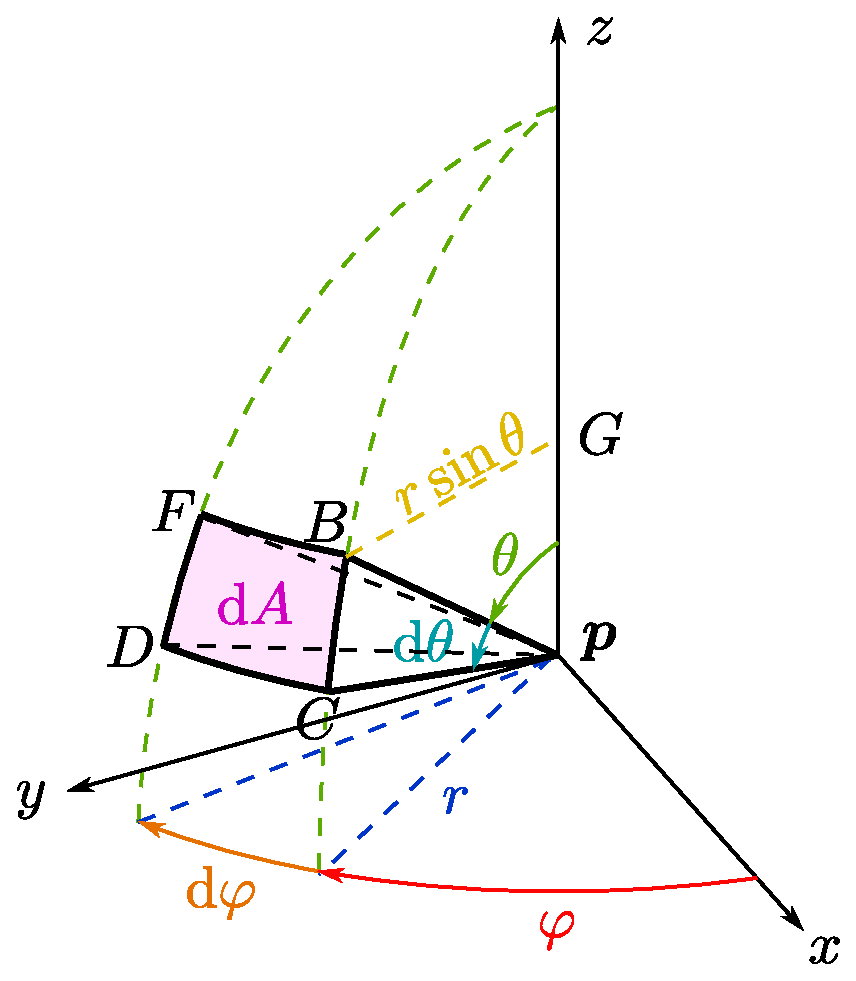
\includegraphics[width=0.4\linewidth]{chap05/ex-solidangle.eps}
      \caption{立体角的定义。}
      \label{fig:5.ex01}
\end{figure}

立体角常用字母$\varOmega$表示。\reffig{5.ex01}展示了一种简单的情形。
以$\bm p$为顶点的微分锥体${\bm p}-BCDF$在同样以$\bm p$为球心且半径为$r$的球面上截取下微分面$BCDF$。
建立以$\bm p$为原点的球坐标系,则弧线$\wideparen{BC}$的方位角
(在$xy$平面上的投影与原点连线和$x$正半轴所成角)为$\varphi$,
$\wideparen{DF}$方位角为$\varphi+\mathrm{d}\varphi$;
弧线$\wideparen{BF}$的天顶角(与原点连线和$z$正半轴所成角)为$\theta$,
$\wideparen{CD}$的天顶角为$\theta+\mathrm{d}\theta$。
于是易知点$B$到其在$z$轴投影点$G$的距离为$r\sin\theta$,
因此$\wideparen{BF}$的弧长为$r\sin\theta\mathrm{d}\varphi$;
同时$\wideparen{BC}$的弧长为$r\mathrm{d}\theta$。
将微分面$BCDF$视作矩形,可求得其微分面积为
\begin{align}
      \mathrm{d}A=r\sin\theta\mathrm{d}\varphi\cdot r\mathrm{d}\theta\, .
\end{align}
依据定义,则相应的微分立体角为
\begin{align}
      \mathrm{d}\varOmega=\frac{\mathrm{d}A}{r^2}=\sin\theta\mathrm{d}\theta\mathrm{d}\varphi\, .
\end{align}
对微分立体角做曲面积分则可得立体角
\begin{align}
      \varOmega=\iint\limits_S \mathrm{d}\varOmega=\iint\limits_S \sin\theta\mathrm{d}\theta\mathrm{d}\varphi\, .
\end{align}

立体角的单位为\keyindex{球面度}{steradian}{}(sr),是无量纲的导出单位。
\begin{corollary}
      封闭曲面对于其内任意一点的立体角均为$4\pi$sr。
\end{corollary}
